\chapter{Sistema medio}
\label{C:SistemaMedio}


El sistema medio se realizó con el objetivo de implementar una arquitectura más compleja que el sistema mínimo, permitiendo desarrollar programas del tipo dinámico en el sistema. Principalmente, se buscaba implementar programas que interactuaban con la memoria del sistema de forma dinámica, es decir, que utilizaban una memoria del tipo RAM, la cual se utiliza en la arquitectura del sistema medio. La diferencia principal con respecto al sistema mínimo es el uso de toda la memoria disponible en el mapa de memoria, permitiendo implementar códigos que requieren de mayor disponibilidad de memoria y por ende son más complejos. 

El microprocesador CDP1802 cuenta con un direccionamiento de 16 bits, no obstante, el mismo utiliza solamente 8 líneas para el bus de direcciones. La solución presentada por el microprocesador para el direccionamiento es enviar primero los 8 bits más significativos de la dirección, luego los 8 bits menos significativos. Para evitar la pérdida de los 8 primeros bits se debe integrar un latch (74HC373) que almacene los primeros 8 bits del bus de direcciones, y el mismo microprocesador sincroniza al latch con una señal para el registro de los datos. 

Es de esta manera que el sistema medio puede direccionar una mayor cantidad de memoria que en el sistema mínimo (256 x 8), utilizando un latch de 8 bits 74HC373\cite{datasheet_74HC373} y aprovechando el mecanismo propuesto por el CDP1802 para aumentar la cantidad de líneas de dirección hasta 16 bits, logrando direccionar 64k x 8. Esto se observa en el diagrama de bloques de la Figura~\ref{F:diag_bloq_sistema_medio}.

 \begin{figure}[H]
  \centering
  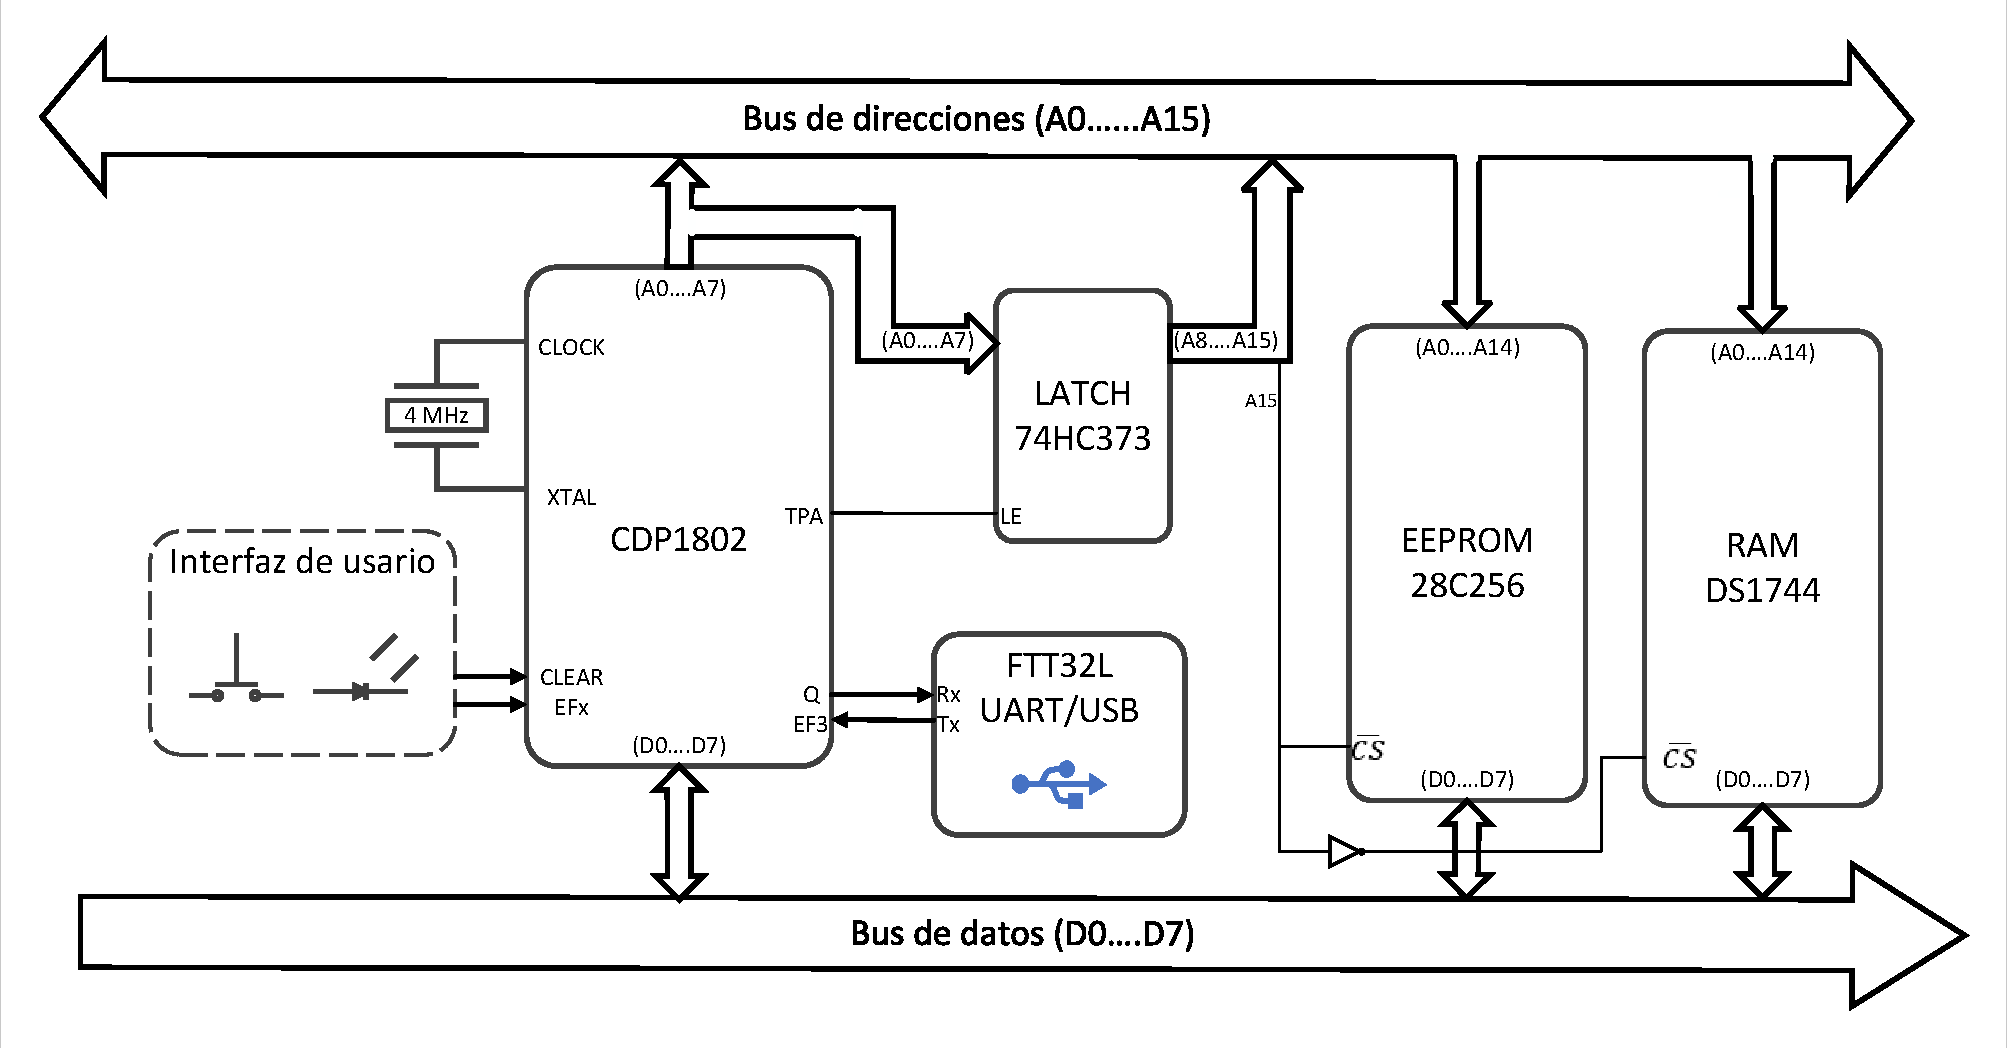
\includegraphics[width=0.98\textwidth]{./imagenes/diag_bloq_sistema_medio.pdf}
  \caption{Diagrama de bloques del sistema medio}
  \label{F:diag_bloq_sistema_medio}
\end{figure}

Esta incorporación de la memoria RAM es la principal diferencia con el sistema mínimo, lo cual se muestra en el mapa de memoria de la Figura~\ref{F:mapa_de_mem_sis_med}, donde se tiene una memoria de programa EEPROM (32k x 8) y una memoria de datos RAM (32k x 8); que en total utilizan toda la capacidad de direccionamiento (64k x 8).

\begin{figure}[ht]
  \centering
  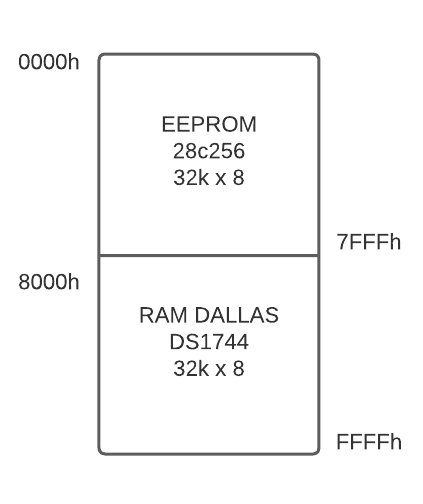
\includegraphics[width=0.4\textwidth]{./imagenes/mapa_de_mem_sis_med.png}
  \caption{Mapa de memoria del sistema medio}
  \label{F:mapa_de_mem_sis_med}
\end{figure}


 
Para realizar la interacción con la terminal externa, se incluyó en el esquema del sistema medio un conversor de UART/USB que dota al sistema de la capacidad de interactuar con una computadora externa, lo cual se explicará mejor en la sección de programas. Los demás dispositivos utilizados son los mismos que en el sistema mínimo y son los requeridos para asegurar el funcionamiento del sistema de forma integral. El esquemático del sistema medio se encuentra en la Figura~\ref{F:esquematico_SME}, el cual fue realizado con el software KiCad. 

 \begin{figure}[ht]
  \centering
  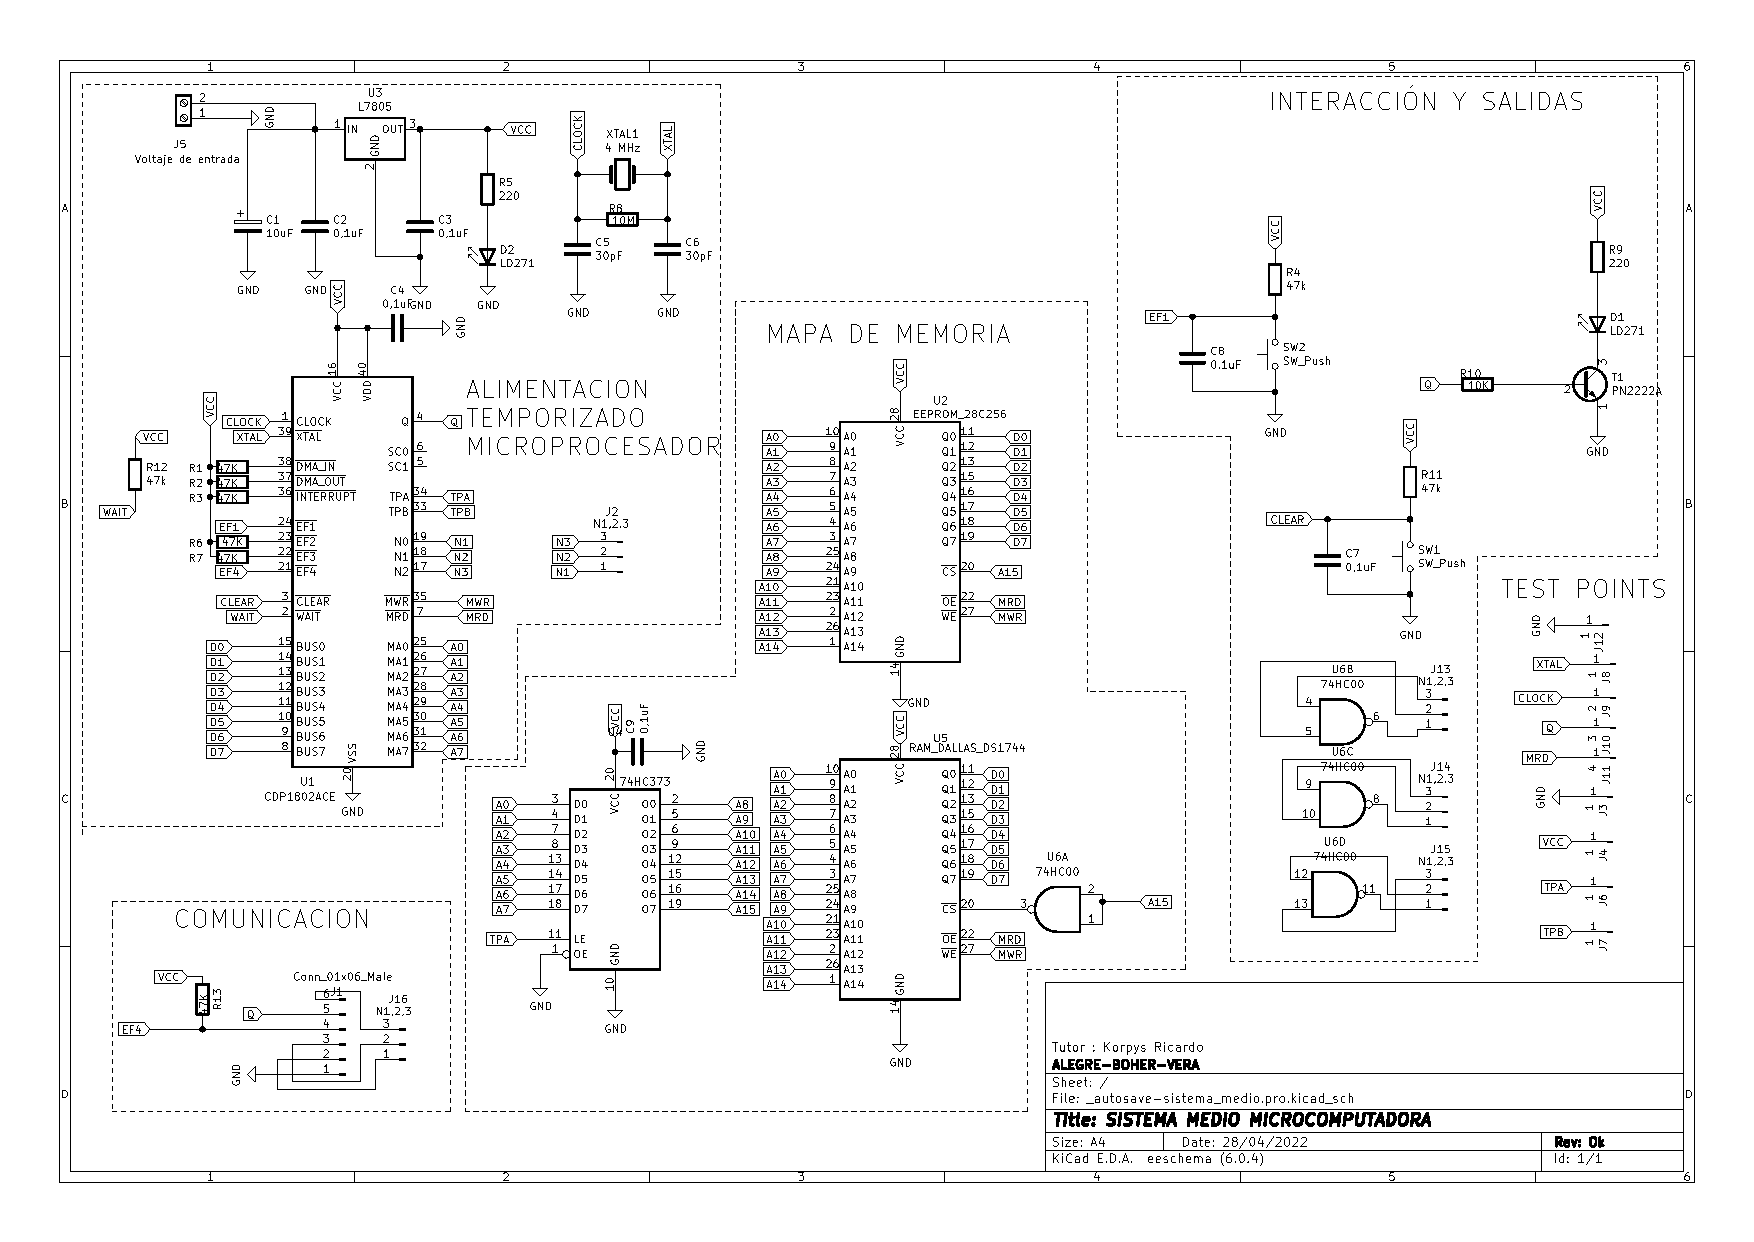
\includegraphics[width=1.20\textwidth, angle=90]{./imagenes/esquematico_SME.pdf}
  \caption{Esquemático del sistema medio}
  \label{F:esquematico_SME}
\end{figure}

 \begin{foto}[ht]
  \centering
  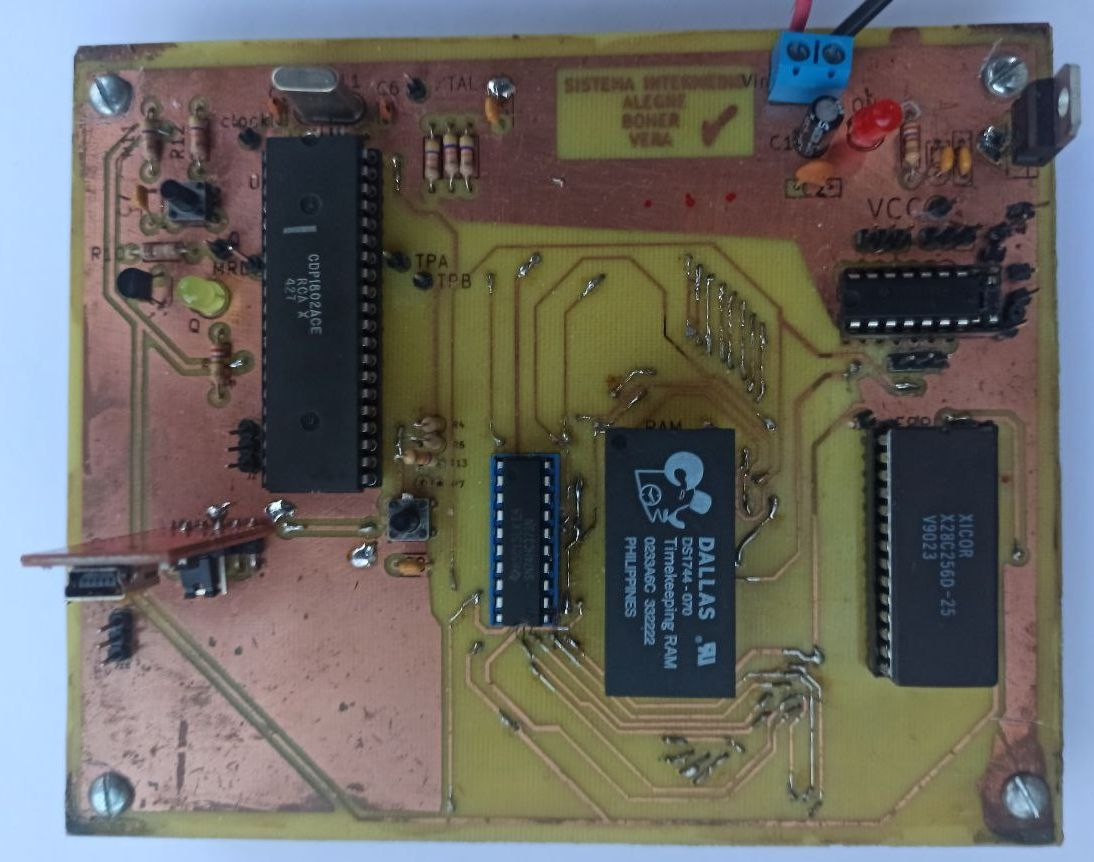
\includegraphics[width=0.9\textwidth]{./imagenes/foto_sistema_med.jpg}
  \caption{Sistema medio construido}
  \label{F:foto_sistema_med}
\end{foto}



\clearpage
\section{Lista de componentes}

En la tabla~\ref{T:bom_sis_med} se encuentra la lista de materiales para la construcción del sistema medio.

\begin{table}[ht!]
\caption{Lista de componentes del sistema medio}
\label{T:bom_sis_med}
\footnotesize
\begin{tabular}{|p{0.08\textwidth}|p{0.11\textwidth}|p{0.30\textwidth}|p{0.14\textwidth}|p{0.15\textwidth}|}
\hline
Cantidad & Etiqueta \newline
           Identificador            & Descripción                               & Fabricante            & Número de parte   \\ \hline \hline
1       & U1                        & Microprocesador                           & RCA                   & CDP1802ACE        \\ \hline
1       & U2                        & Memoria EEPROM 32k x 8                    & XICOR                 & X28C256D-25       \\ \hline
1       & U3                        & Regulador de tensión 5~\si{\volt}         & ST Microelectronics   & L7805CV          \\ \hline
1       & U4                        & Latch de 8 bits                           & Texas Instruments     & SN74HC373N        \\ \hline
1       & U5                        & Time keeping RAM 32K x8                   & Dallas                & DS1744-070        \\ \hline
1       & U6                        & Quadruple 2-Input NAND Gates              & Texas Instruments     & SN74HC00N         \\ \hline
1       & T1                        & Transistor BJT NPN                        & ST Microelectronics   & PN2222A           \\ \hline
1       & XTAL1                     & Cristal \num{4}~\si{\mega\hertz}          & CQ Electronics        & \listaVacio                \\ \hline
2       & SW1, SW2                  & Pulsador 6mm~x~4,3mm                      &  \listaVacio                     &  \listaVacio               \\ \hline
9      & R1, R2, R3, R4, R6, R7, R11, R12, R13
                                    & Resistor 47~\si{\kilo\ohm} 1/8~\si{\watt} &     \listaVacio                  &     \listaVacio            \\ \hline
2       & R5, R9                        & Resistor 220~\si{\ohm} 1/4~\si{\watt}     &      \listaVacio                 &   \listaVacio              \\ \hline
1       & R8                        & Resistor 10~\si{\mega\ohm} 1/8~\si{\watt} &    \listaVacio                   &      \listaVacio           \\ \hline
1       & R10                       & Resistor 10~\si{\kilo\ohm} 1/8~\si{\watt} &  \listaVacio                     &    \listaVacio             \\ \hline
1       & D1                        & LED Rojo 5mm                              &  \listaVacio                     &  \listaVacio               \\ \hline
1       & D2                        & LED Verde 5mm                             &   \listaVacio                    &  \listaVacio               \\ \hline
1       & C1                        & Capacitor electrolítico 10~\si{\micro\farad} 25~\si{\volt}
                                                                                & \listaVacio                      &  \listaVacio               \\ \hline
6       & C2, C3, C4, C7, C8, C9    & Capacitor cerámico \num{0.10}~\si{\micro\farad} 50~\si{\volt}
                                                                                &  \listaVacio                     &   \listaVacio              \\ \hline
2       & C5, C6                    & Capacitor cerámico \num{30}~\si{\pico\farad} 50~\si{\volt}
                                                                                & \listaVacio                      & \listaVacio                \\ \hline
1       & J1                        & 1x6 Pines Conectores Macho \num{2.54}~mm  &  \listaVacio                     &   \listaVacio              \\ \hline
5       & J2, J13, J14, J15, J16    & 1x3 Pines Conectores Macho \num{2.54}~mm  &  \listaVacio                     &  \listaVacio               \\ \hline
9       & J3, J4, J6, J7, J8, J9, J10, J11, J12
                                    & Pin conector macho (1 \textit{Male Header Pin})
                                                                                &  \listaVacio                     &  \listaVacio               \\ \hline
1       & J5                        & Bornera 2 pines \num{5.08}~mm             &  \listaVacio                     &  \listaVacio               \\ \hline
1       & No aplica                 & Módulo conversor USB-Serial               & Future Technology Devices International & FT232RL \\ \hline
\end{tabular}
\normalsize
\end{table}


\clearpage
\section{Programas del sistema medio}
\label{C:programas_del_sistema_medio}

Los programas realizados para el sistema mínimo, expuestos en la sección~\ref{C:ProgramasSMin}, son compatibles con el sistema medio, salvo el programa número~4, que requiere un ajuste en el contador utilizado para la rutina de retardo, debido a que el sistema medio utiliza un cristal de 4~\si{\mega\hertz} ($ T_{reloj} = \num{250}~\si{\nano\second} $), distinto al utilizado en el sistema mínimo. Para su cálculo, utilizamos la ecuación~\eqref{eq:contador}, expuesta en la sección~\ref{C:ComunicacionSerial}, y considerando, al igual que en el sistema mínimo, 600~baudios (Retardo = \num{0.001666667}~\si{\second}).

\begin{equation}
    CONT1BT = \frac{Retardo}{48\:T_{reloj}}-\frac{4}{3} = \frac{\num{0.001666667}~\si{\second}}{48\cdot\num{250}~\si{\nano\second}}-\frac{4}{3} = \num{137.56}\approx\num{138}
    \label{eq:calculo-1-bit-time-sistema-med}
\end{equation}

A continuación, se exponen otros programas implementados en el sistema medio.

\subsection{Intérprete Tiny Basic}

En la página oficial del Membership Card\cite{membership-card} puede encontrarse un intérprete Basic bajo el nombre de Tiny BASIC. El mismo tiene documentación y el código fuente, lo cual resulta de gran ayuda. Sin embargo, para su correcto funcionamiento en el sistema medio, es necesario realizar una serie de modificaciones en el código fuente.

La primera de estas modificaciones es en el archivo \texttt{1802reg.asm}, el cual contiene definido el nombre de los registros de trabajo. Sin embargo, faltaban algunos registros y fue necesario agregarlos. Para que el código pueda ser ensamblado sin errores, es necesario que este archivo tenga todas las definiciones que se encuentran en el código del listado~\ref{L:1802reg}.

\clearpage
\footnotesize
\lstinputlisting[language=CDP1802, caption={\centering Archivo \texttt{1802reg.asm} con definición de etiquetas para los registros de trabajo}, label = {L:1802reg}]{codigo/1802reg.asm}
\normalsize

Las siguientes modificaciones se realizaron sobre el código fuente del intérprete Tiny BASIC, más específicamente, el archivo \texttt{tb0\_test.asm}. Este código es muy extenso para ser incluido en este informe, sin embargo, se incluyen segmentos pequeños del código, donde pueden visualizarse las modificaciones realizadas.

La segunda modificación fue realizada en la línea 25, que puede verse en el listado~\ref{L:basic_mod1_starts_at_1}, donde la etiqueta \texttt{QHI} debe ser definida como 0, esto es necesario para que la línea de transmisión serial a través del pin Q, cuando esté en reposo, sin trasmitir datos, permanezca en estado alto, como lo establece el protocolo UART. Y la última modificación realizada, esta vez en la línea 28 del listado~\ref{L:basic_mod1_starts_at_1}, fue definir la etiqueta \texttt{AUTORUN} como 0; si esta etiqueta permanece definida como 1, al iniciar el intérprete, se ejecuta un código predefinido, lo cual en ocasiones resulta molesto, por lo que se decidió desactivar esta opción.

\footnotesize
\lstinputlisting[language=CDP1802, caption={\centering Segmento del código fuente \texttt{tb0\_test.asm} con modificación en línea 25 y 28}, label = {L:basic_mod1_starts_at_1}]{codigo/basic_mod1_starts_at_1.asm}
\normalsize

Estas son todas las modificaciones realizadas. Sin embargo, existen partes de interés en el código que vale la pena mencionar, a pesar de que no fueron modificadas. La primera de ellas se encuentra en la línea~91 del código, listado~\ref{L:basic_mod2_starts_at_89}, donde se encuentra definida la etiqueta \texttt{PAGE}, que define la posición de la memoria RAM en el mapa de memoria, empezando en este caso a partir de 8000~hexadecimal. Para el funcionamiento en el sistema medio no es necesario modificar esta etiqueta, sin embargo, en otras arquitecturas sí puede ser necesario.

\clearpage
\footnotesize
\lstinputlisting[language=CDP1802, caption={\centering Segmento del código fuente \texttt{tb0\_test.asm}, modificación de posición de memoria RAM en el mapa de memoria}, firstnumber=89, label = {L:basic_mod2_starts_at_89}]{codigo/basic_mod2_starts_at_89.asm}
\normalsize

Finalmente, en la línea~2194 del código, listado~\ref{L:basic_set_baudrate_starts_at_2187}, puede modificarse la velocidad de transmisión (baudrate). Por defecto es de \num{2400}~baudios para el caso del sistema medio, que utiliza un cristal de \num{4}~\si{\mega\hertz}.

\footnotesize
\lstinputlisting[language=CDP1802, caption={\centering Segmento del código fuente \texttt{tb0\_test.asm}, definición del baudrate utilizado con cristal de \num{4}~\si{\mega\hertz}}, firstnumber=2187, label = {L:basic_set_baudrate_starts_at_2187}]{codigo/basic_set_baudrate_starts_at_2187.asm}
\normalsize

\subsection{Sistema operativo ElfOS sin disco}

En la página oficial del Membership Card\cite{membership-card} puede encontrarse una versión del sistema operativo ElfOS sin disco (en la página el término en inglés es \entreComillas{Diskless Elf/OS ROM}). Desafortunadamente, el código fuente de este programa no se encuentra disponible, solo un archivo \texttt{.hex}. Esto significa que no es posible modificar el programa, pero puede ser grabado en una memoria y utilizado en el sistema medio.

Este sistema operativo inicia presentando un menú donde puede seleccionarse una serie de programas, en la figura~\ref{F:menu_del_elfOS} pueden visualizarse todos los programas disponibles.

 \begin{figure}[ht]
  \centering
  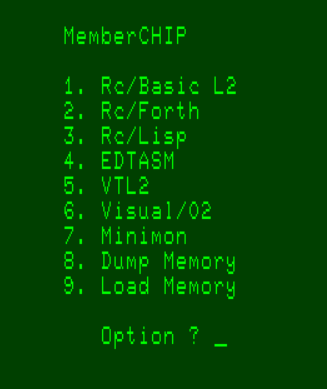
\includegraphics[width=0.35\textwidth]{./imagenes/menu_del_elfOS.png}
  \caption{Menú del sistema operativo ElfOS sin disco}
  \label{F:menu_del_elfOS}
\end{figure}

\clearpage
\section{Simulación Emma02}

\subsection{Intérprete Tiny Basic}

El intérprete Tiny Basic fue ejecutado correctamente en el simulador Emma02, utilizando el Membership Card, en la figura~\ref{F:config_emma_sis_med} puede apreciarse la configuración utilizada. Algo a ser destacado es que para la transmisión serial de datos, la configuración utilizada en el simulador es de 8 bits para el dato y sin bit de paridad, sin embargo, utilizando el sistema medio construido, se encontró que la configuración debe ser distinta; esta configuración se encuentra detallada en la sección~\ref{C:int_basic_resul_exper}.

 \begin{figure}[ht]
  \centering
  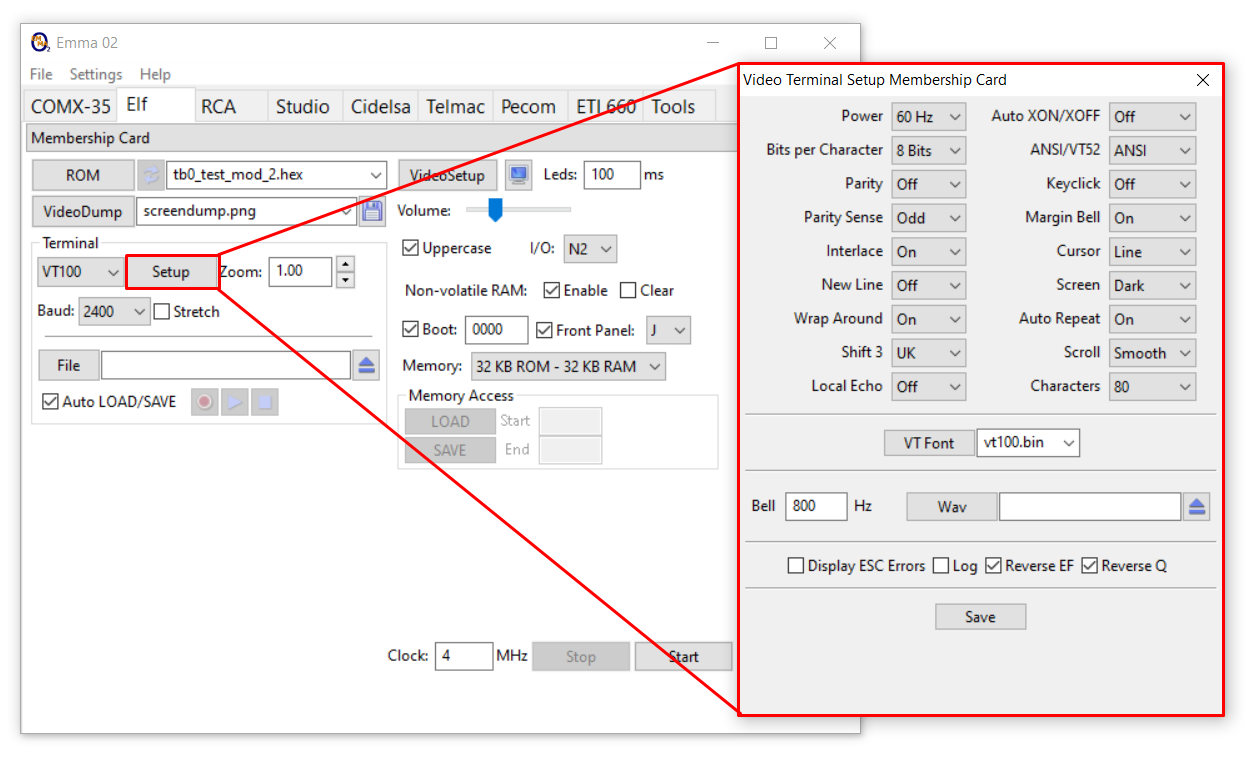
\includegraphics[width=1\textwidth]{./imagenes/config_emma_sis_med.png}
  \caption{\centering Configuración utilizada en el simulador Emma02 para ejecutar el intérprete Tiny Basic y el ElfOS sin disco}
  \label{F:config_emma_sis_med}
\end{figure}

\subsection{Sistema operativo ElfOS sin disco}

El sistema operativo ElfOS sin disco también fue ejecutado correctamente en el simulador Emma02, de nuevo utilizando el Membership Card con la misma configuración expuesta en la figura~\ref{F:config_emma_sis_med}.

\section{Resultados experimentales}

\subsection{Intérprete Tiny Basic}
\label{C:int_basic_resul_exper}

El intérprete Basic fue probado en el sistema medio, habiendo obtenido los mismos resultados que con el simulador Emma02. Sin embargo, para poder funcionar correctamente, fue necesario utilizar una configuración distinta para la comunicación serial. A continuación, se describe la misma.

Para la comunicación serial se utilizó una velocidad de 2400~baudios, 7 bits para los datos, bit de paridad impar y dos bits de stop, Flow Control en none, y transmit delay nulo.


\subsection{Sistema operativo ElfOS sin disco}

El sistema operativo ElfOS sin disco pudo ejecutarse correctamente en el sistema medio. La configuración para la comunicación serial fue la siguiente: Velocidad de 2400~baudios, 8~bits para los datos, sin bit de paridad y dos bits de stop, Flow Control en none, y transmit delay nulo.
